\documentclass[a4paper]{article}
\usepackage[pdftex]{hyperref}
\usepackage[latin1]{inputenc}
\usepackage[english]{babel}
\usepackage{a4wide}
\usepackage{amsmath}
\usepackage{amssymb}
\usepackage{algorithmic}
\usepackage{algorithm}
\usepackage{ifthen}
\usepackage{listings}
\usepackage{array}
\usepackage{tabu}
% move the asterisk at the right position
\lstset{basicstyle=\ttfamily,tabsize=4,literate={*}{${}^*{}$}1}
%\lstset{language=C,basicstyle=\ttfamily}
\usepackage{moreverb}
\usepackage{palatino}
\usepackage{multicol}
\usepackage{tabularx}
\usepackage{comment}
\usepackage{verbatim}
\usepackage{color}
\usepackage{graphicx}

%% pdflatex?
\newif\ifpdf
\ifx\pdfoutput\undefined
\pdffalse % we are not running PDFLaTeX
\else
\pdfoutput=1 % we are running PDFLaTeX
\pdftrue
\fi
\ifpdf
\fi
\ifpdf
\DeclareGraphicsExtensions{.pdf, .jpg}
\else
\DeclareGraphicsExtensions{.eps, .jpg}
\fi

\parindent=0cm
\parskip=0cm

\setlength{\columnseprule}{0.4pt}
\addtolength{\columnsep}{2pt}

\addtolength{\textheight}{5.5cm}
\addtolength{\topmargin}{-26mm}
\pagestyle{empty}

%%
%% Sheet setup
%% 
\newcommand{\coursename}{Computer Architecture and Programming Languages}
\newcommand{\courseno}{CO20-320241}
 
\newcommand{\sheettitle}{Homework}
\newcommand{\mytitle}{}
\newcommand{\mytoday}{{30 September}, 2019}

% Current Assignment number
\newcounter{assignmentno}
\setcounter{assignmentno}{3}

% Current Problem number, should always start at 1
\newcounter{problemno}
\setcounter{problemno}{1}

%%
%% problem and bonus environment
%%
\newcounter{probcalc}
\newcommand{\problem}[2]{
  \pagebreak[2]
  \setcounter{probcalc}{#2}
  ~\\
  {\large \textbf{Problem \textcolor{blue}{\arabic{assignmentno}}.\textcolor{blue}{\arabic{problemno}}} \hspace{0.2cm}\textit{#1}} \refstepcounter{problemno}\vspace{2pt}\\}

\newcommand{\bonus}[2]{
  \pagebreak[2]
  \setcounter{probcalc}{#2}
  ~\\
  {\large \textbf{Bonus Problem \textcolor{blue}{\arabic{assignmentno}}.\textcolor{blue}{\arabic{problemno}}} \hspace{0.2cm}\textit{#1}} \refstepcounter{problemno}\vspace{2pt}\\}

%% some counters  
\newcommand{\assignment}{\arabic{assignmentno}}

%% solution  
\newcommand{\solution}{\pagebreak[2]{\bf Solution:}\\}

%% Hyperref Setup
\hypersetup{pdftitle={Homework \assignment},
  pdfsubject={\coursename},
  pdfauthor={},
  pdfcreator={},
  pdfkeywords={Computer Architecture and Programming Languages},
  %  pdfpagemode={FullScreen},
  %colorlinks=true,
  %bookmarks=true,
  %hyperindex=true,
  bookmarksopen=false,
  bookmarksnumbered=true,
  breaklinks=true,
  %urlcolor=darkblue
  urlbordercolor={0 0 0.7}
}

\begin{document}
\coursename \hfill Course: \courseno\\
Jacobs University Bremen \hfill \mytoday\\
Fjolla Dedaj\hfill
\vspace*{0.3cm}\\
\begin{center}
{\Large \sheettitle{} \textcolor{blue}{\assignment}\\}
\end{center}

\problem{}{0}
\solution
\\
Distributive Law: DL\\
Identity Law: IL\\
Annulment Law: AL\\
Complement Law: CL\\
De Morgan's Theorem: DM\\
Double Negation Law: DN\\
\\
\textbf{a)} \\
$x=(M+N)(\overline{M}+P)(\overline{N}+\overline{P}) = \\
\\
DL: = (M\overline{M} + MP + N\overline{M}+NP)(\overline{N}+\overline{P})=\\
\\
IL: = (MP+ N\overline{M}+NP)(\overline{N}+\overline{P})=\\
\\
DL: = MP\overline{N} + MP\overline{P} + N\overline{M}\overline{N} + N\overline{M}\overline{P} + NP\overline{N} + NP\overline{P}\\
\\
IL: = M\overline{N}P + \overline{M}N\overline{P}
$
\\
\\
\textbf{b)}\\
$z=\overline{A}B\overline{C}+AB\overline{C}+B\overline{C}D = \\
\\
DL: = B\overline{C}(\overline{A} + A + D) = \\
\\
CL: = B\overline{C}(1 + D) = \\
\\
AL: = B\overline{C}$\\ 
\\
\textbf{c)}\\ 
$x=\overline{(M+N+P)Q} = \\
\\
DM: = \overline{M+N+P} + \overline{Q} = \\
\\
DM: = \overline{M} * \overline{N} * \overline{P} + \overline{Q}\\ 
$
\\
\textbf{d)}\\
$z=\overline{ABC+DEF} = \\
\\
DM: = \overline{ABC} * \overline{DEF} =\\
\\
DM: = (\overline{A} + \overline{B} + \overline{C}) * (\overline{D} + \overline{E} + \overline{F})\\\
$
\\
\textbf{e)}\\
$z=\overline{A\overline{B} +C\overline{D} + EF} =\\
\\
DM: = \overline{A\overline{B}} * \overline{C\overline{D}} * \overline{EF} =\\
\\
DM: =(\overline{A} + \overline{\overline{B}}) * (\overline{C} + \overline{\overline{D}}) * (\overline{E} + \overline{F}) =\\
\\
DN: = (\overline{A} + B) * (\overline{C} + D) * (\overline{E} + \overline{F})
\\
$
\\
\pagebreak
\\
\textbf{f)}\\ 
Throughout this problem, we use De Morgan's Theorem in every step and DN in some of the steps where we have double negation:\\ 
\\
$z=\overline{\overline{A + B\overline{C}} + D\overline{(E + \overline{F})}} = \\
\\
= \overline{\overline{A+B\overline{C}}} * \overline{D*(E+\overline{F})}=\\
\\
= \overline{\overline{A} * \overline{B*\overline{C}}} * \overline{D*\overline{E}*\overline{\overline{F}}} = \\
\\
= \overline{\overline{A}*(\overline{B} + \overline{\overline{C}})} * \overline{D\overline{E}F} = \\
\\
= \overline{\overline{A} * (\overline{B}+C)} * (\overline{D\overline{E}F}) =\\
\\
= (\overline{A} + \overline{\overline{B} + C}) * (\overline{D} + \overline{\overline{E}} + \overline{F}) =\\
\\
= (A + \overline{\overline{B}}*\overline{C}) * (\overline{D} + E + \overline{F}) =\\
\\
=(A + B * \overline{C}) * (\overline{D} + E + \overline{F})\\
$
\\
\problem{}{0}
\solution
\\
Firstly, we obtain the following boolean expression from analyzing the circuit:\\
\\
$x = (\overline{A} \wedge \overline{B} \wedge D) \vee (A \wedge \overline{B} \wedge \overline{C}) \vee (\overline{A} \wedge \overline{B} \wedge \overline{C})$\\
\\
Now, from the expression above, we can create the Karnaugh Map by using gray encoding and plotting the 1s correspondingly.
\\
\\
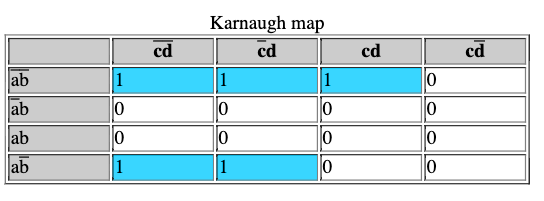
\includegraphics[scale=0.6]{table.png}
\\
\\
After grouping the 1s in three different groups (two groups with two 1s and a group with a single 1) and analyzing the Karnaugh Map, we get the following simplified boolean expression: $\overline{A}\overline{B}D + \overline{B}\overline{C}$\\
\pagebreak
\\
\problem{}{0}
\solution
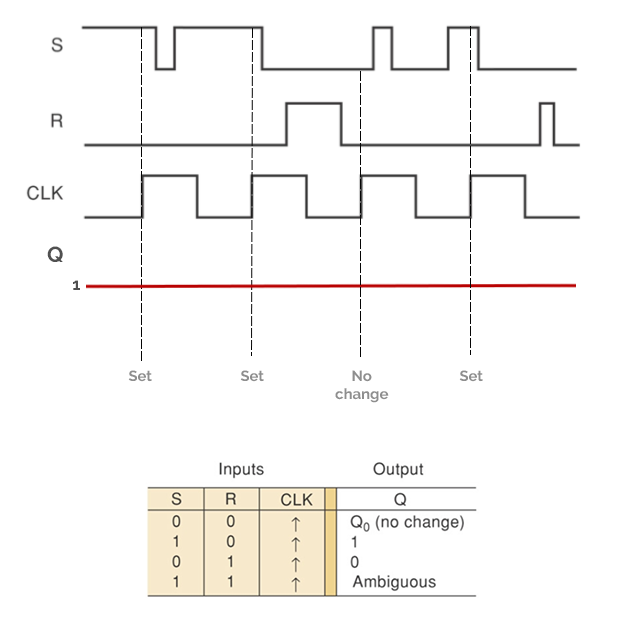
\includegraphics[scale=0.5]{33.png}\\
\\


\problem{}{0}
\solution
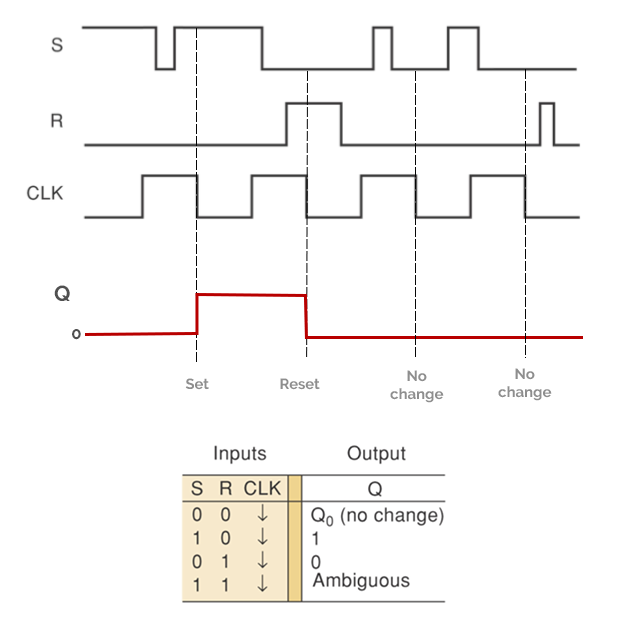
\includegraphics[scale=0.5]{34.png}\\
\pagebreak
\problem{}{0}
\solution
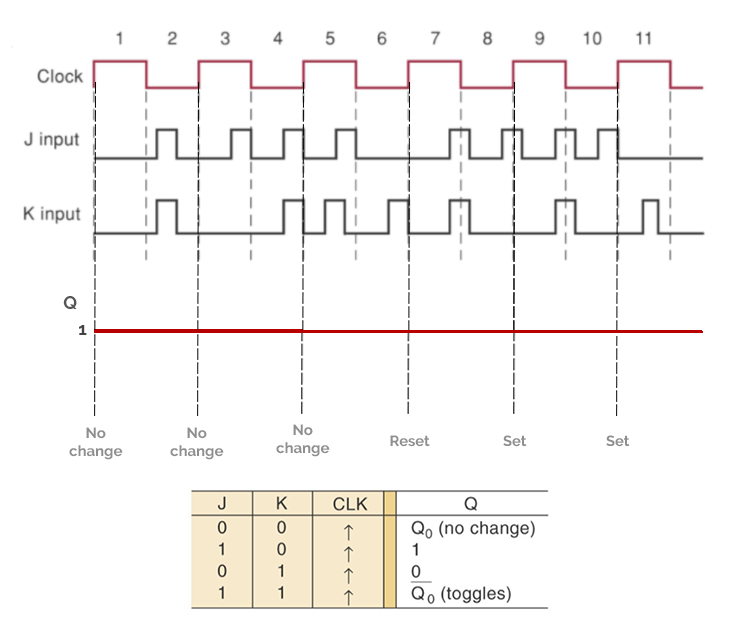
\includegraphics[scale=0.5]{35.png}\\

\problem{}{0}
\solution
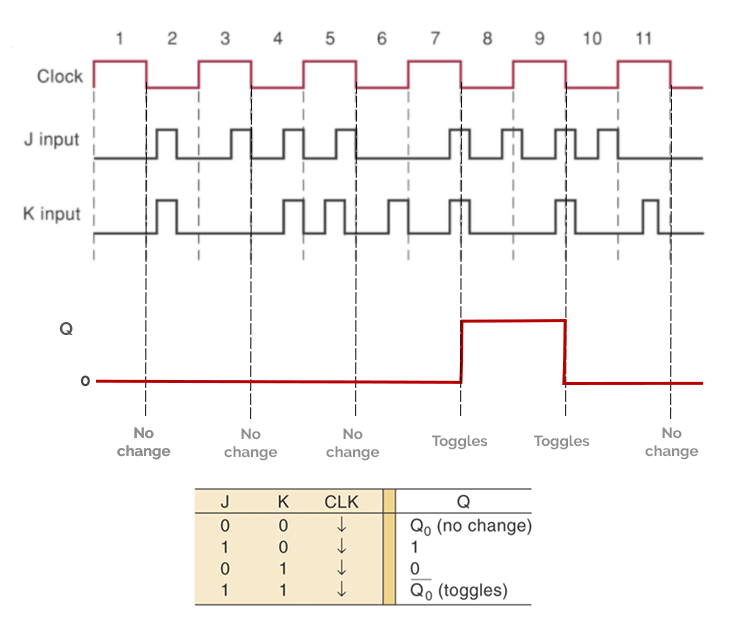
\includegraphics[scale=0.5]{36.png}\\
\pagebreak
\problem{}{0}
\solution
\\
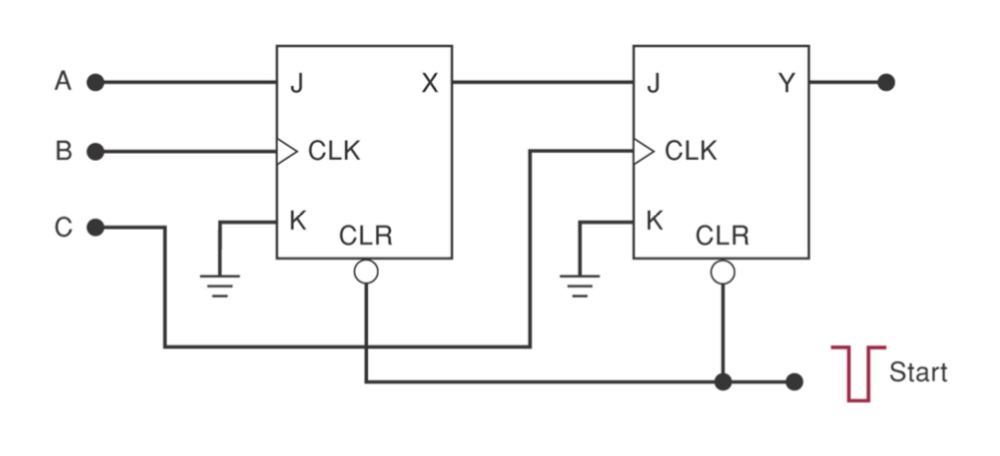
\includegraphics[scale=0.3]{circuit.png}
\\
\textbf{a)}\\
The sequence that makes Y go HIGH is A, B, C because Y can go HIGH only when C goes HIGH while X is already HIGH. X can go HIGH only if B goes HIGH while A is HIGH.\\
\\
\textbf{b)} Need for Start Pulse\\
We know that the outputs X and Y need to be cleared to 0 before applying the A, B and C signals. To clear the outputs, we need a negative going Start pulse at the R input. R of JK flip-flop is active LOW.
\\
\\
\textbf{c)}\\
A D Flip-Flop may be implemented with a J-K Flip-Flop by tying the J input to the K input through an inverter, as it is shown below:\\
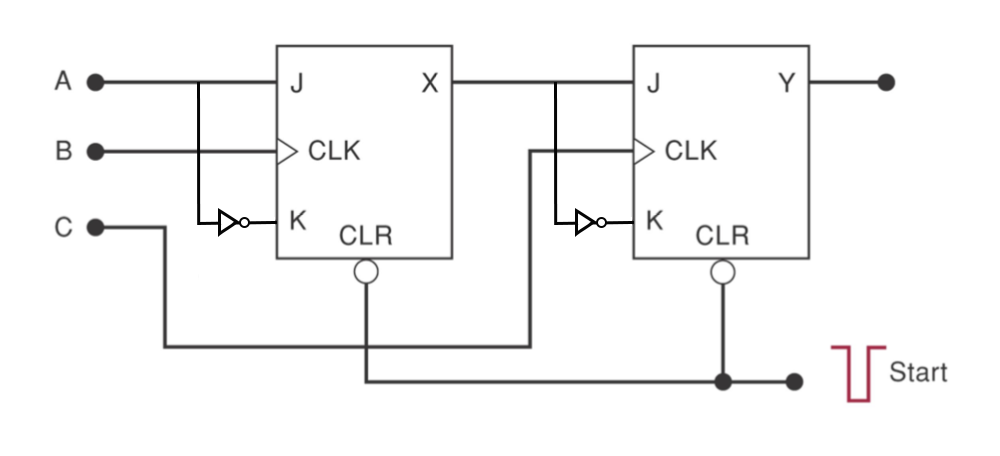
\includegraphics[scale=0.3]{circuit2.png}
\\
\\
which is equivalent to:\\
\\
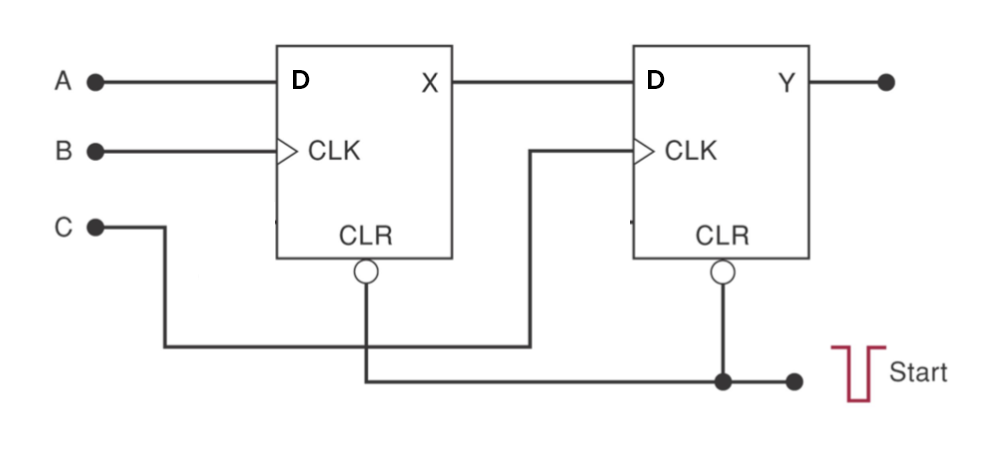
\includegraphics[scale=0.3]{circuit3.png}

\end{document}